\usetikzlibrary{decorations.pathreplacing}
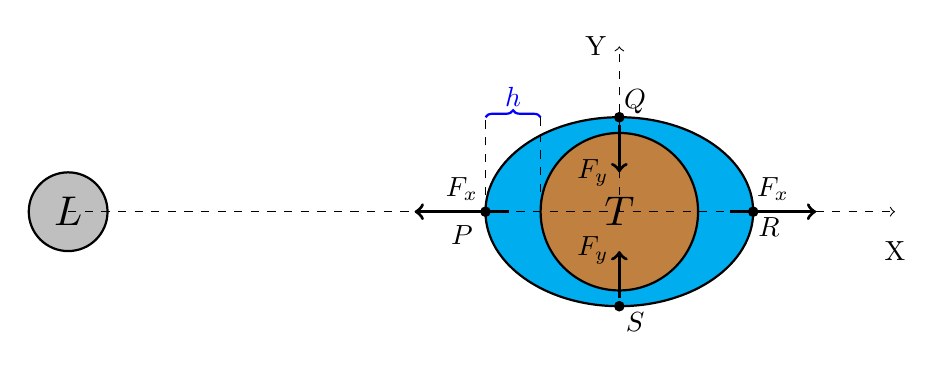
\begin{tikzpicture}
\draw  [thick, fill=cyan] (1.5,0.5) node (v1){} ellipse (1.7 and 1.2);
\draw  [thick, fill=brown](v1) circle (1);
\draw [thick, fill=lightgray] (-5.5,0.5) circle (0.5)node [scale=1.5] (v2) {$L$};
\node [scale=1.5] at (1.5,0.5) {$T$};

\node at (-0.5,0.2) {$P$};
\node at (1.7,-0.9) {$S$};
\node at (3.4,0.3) {$R$};
\node at (1.7,1.9) {$Q$};
\draw [dashed, ->](v2.center) -- (5,0.5);
\node at (5,0) {X};
\draw [decorate, decoration=brace, draw=blue, thick](-0.2,1.7) -- (0.5,1.7)node [midway, above, blue]{$h$};
\draw [dashed, ->](v1.center) -- (1.5,2.6);
\node at (1.2,2.6) {Y};
\draw [fill] (1.5,-0.7) circle (0.06);
\draw [fill] (3.2,0.5) circle (0.06);
\draw [fill] (1.5,1.7) circle (0.06);
\draw [fill] (-0.2,0.5) circle (0.06);
\draw [dashed, ultra thin](-0.2,0.5) -- (-0.2,1.7);
\draw [dashed, ultra thin](0.5,1.7) -- (0.5,0.5);
\draw [very thick, ->](0.1,0.5) -- (-1.1,0.5)node[midway, above]{$F_x$};
\draw [very thick, ->](1.5,1.6) -- (1.5,1)node[midway, below left]{$F_y$};
\draw [very thick, ->](1.5,-0.6) -- (1.5,0)node[midway, above left]{$F_y$};
\draw [very thick, ->](2.9,0.5) -- (4,0.5)node[midway, above]{$F_x$};
\end{tikzpicture}